\section{Descripción detallada de la solución informática desarrollada}

Se ha desarrollado un sistema capaz de extraer información de documentos.
Para el desarrollo se ha seguido un conjunto de buenas prácticas cómo por ejemplo el uso de arquitecturas límpias,
esto facilita que la solución pueda ser extendida, para diferentes casos de uso.

El sistema tiene un primer componente, el componente \textit{Generator} con capacidad para convertir documentos
\textbf{PDF} en texto, tal y como definimos en el \textbf{Requisito 1}.

Aunque en esta implementación se han utilizado un sistema concreto para la conversión de documentos \textbf{PDF}
en texto, el sistema permite incorporar otras implementaciones, que hagan la conversión utilizando otros elementos de
infraestructura, o añadiendo soporte para otros formatos.

El sistema tiene un segundo componente, el componente \textit{Reader} capaz de extraer información a partir de la
salida del componente anterior.
Se han implementado el soporte para dos tipos de documento concretos que son los contratos de arrendamiento de vivienda
entre particulares \textbf{Requisito 2} y contratos de compraventa de vehículo entre particulares \textbf{Requisito 3}.

De la misma forma, que con el componente anterior, es sencillo añadir soporte para nuevos tipos de documentos.

Aunque el sistema, está diseñado para usarse en modo librería, integrado dentro de otros sistemas, se desarrollaron
dos interfaces.

La interfaz web está desarrollada en un formato responsive.
Al arrastrar y soltar un documento sobre el cuadro de diálogo, la web mostrará un mensaje con los datos del
documento en formato JSON.

En la figura~\ref{fig:chapter_5.1.web_interface} puede verse el resultado de ejecutar un contrato de arrendamiento
de vivienda entre particulares.

\begin{figure}[ht]
    \begin{center}
        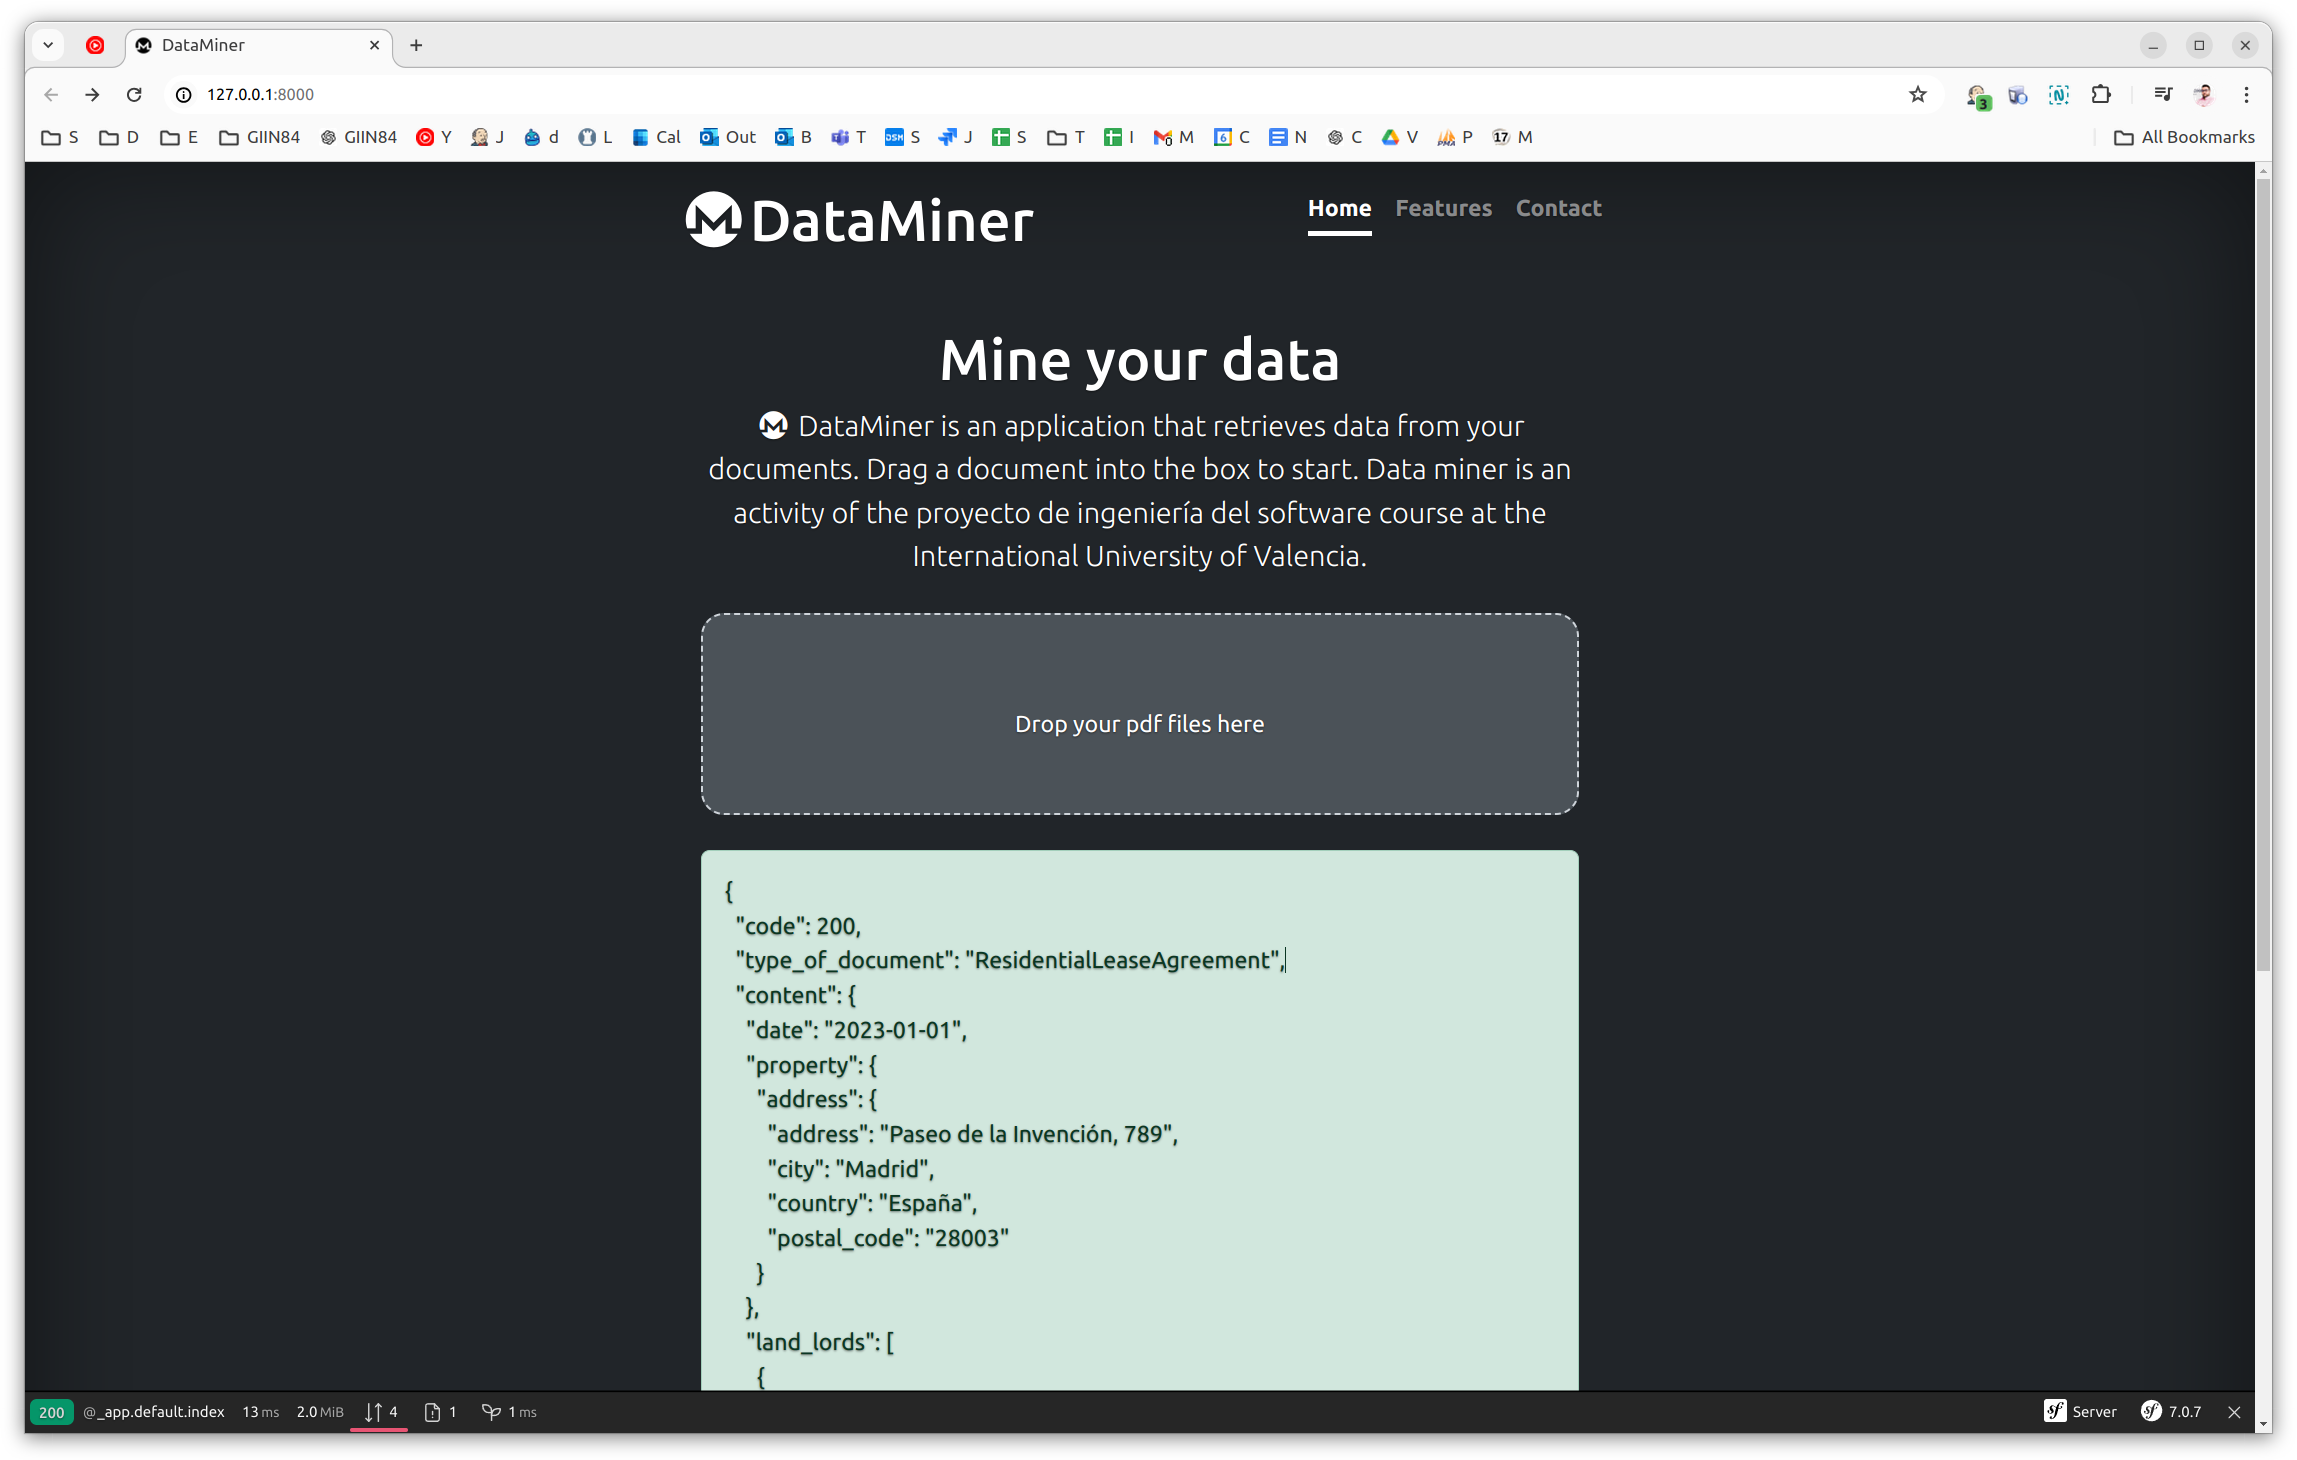
\includegraphics[width=\textwidth]{./chapter/5/images/chapter_5.1.web_interface}
        \caption{Resultado de la ejecución de un documento sobre la interfaz web}
        \label{fig:chapter_5.1.web_interface}
    \end{center}
\end{figure}

La interfaz de línea de comandos, está desarrollada de forma que hay que pasar por parámetro la ruta al documento.
En la figura~\ref{fig:chapter_5.1.cli_interface} puede verse el resultado de ejecutar un contrato de compraventa de
vehículo entre particulares.

\begin{figure}[ht]
    \begin{center}
        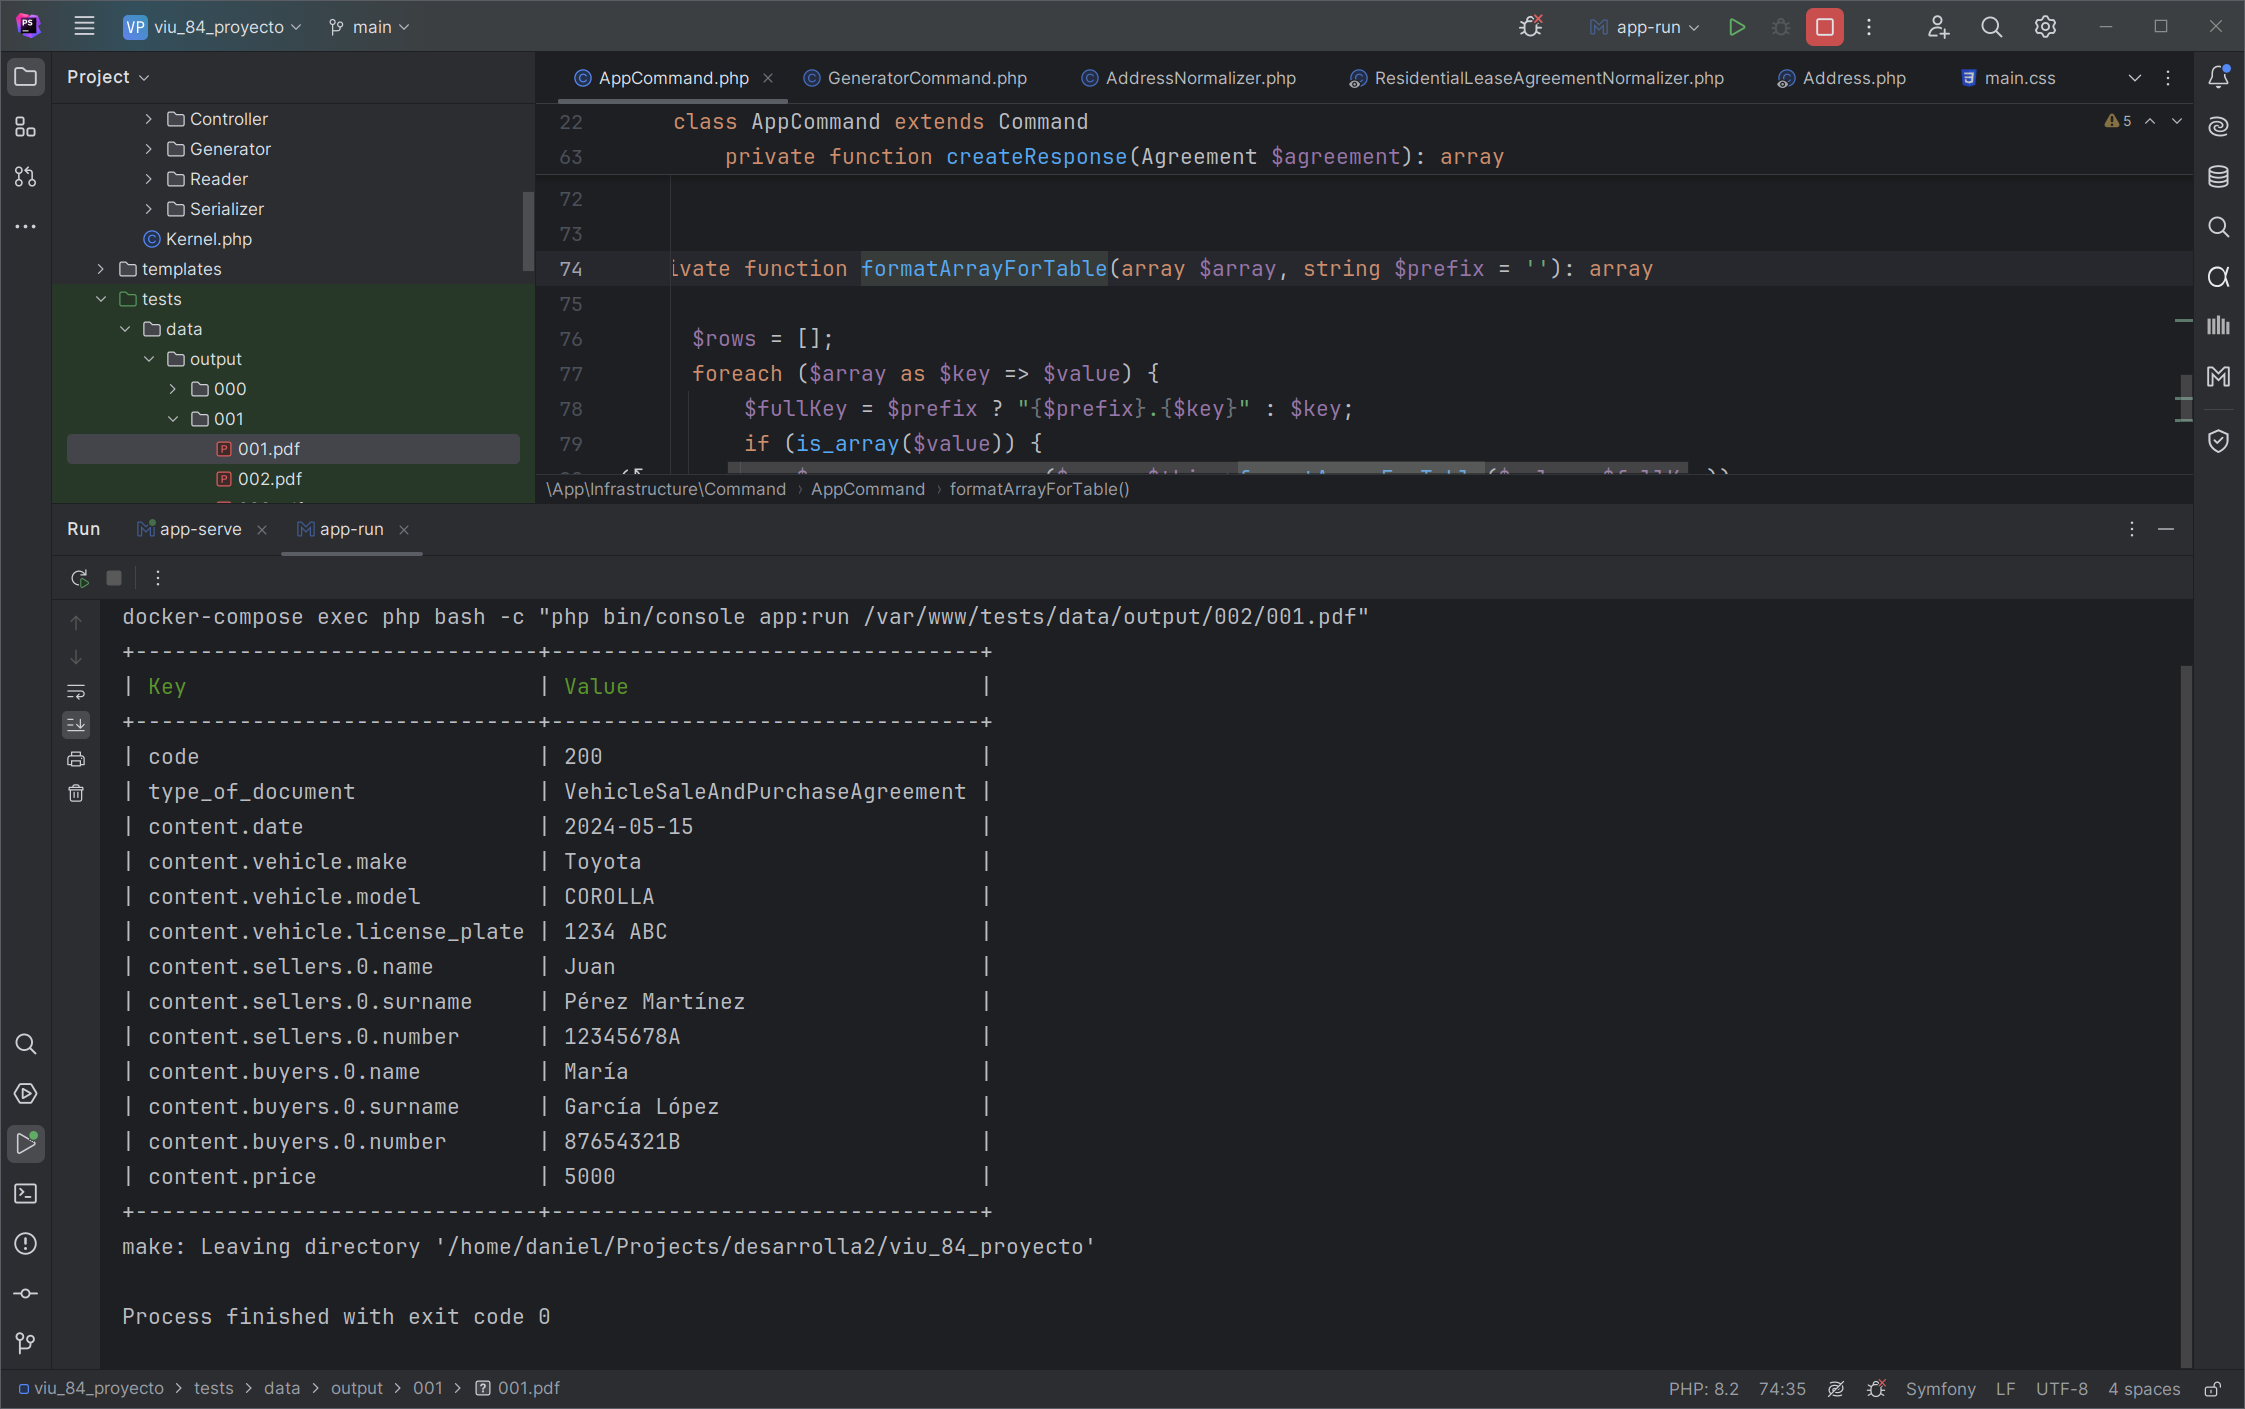
\includegraphics[width=\textwidth]{./chapter/5/images/chapter_5.1.cli_interface}
        \caption{Resultado de la ejecución de un documento sobre la interfaz de línea de comandos}
        \label{fig:chapter_5.1.cli_interface}
    \end{center}
\end{figure}
